\chapter{Métodos Iterativos para Zeros de Função}

Em muitas aplicações, as soluções buscadas se resumem a encontrar os zeros (ou raízes) de uma função. Entretanto, nem sempre é possível fazê-lo analiticamente, devido à natureza das componentes envolvidas na função como, por exemplo, funções polinomiais a partir do 3º grau, somas de funções trigonométricas e logarítmicas, entre outras. Nesse ínterim, recorremos então a maneiras de obter valores aproximados para tais raízes. 

Uma classe de métodos utilizados para aproximar raízes de funções são os \textbf{métodos iterativos}. A essência desses métodos está em, partindo de um chute inicial e de uma função apropriada $\varphi$, obter uma sequência $x_k$ onde cada termo é obtido do anterior recursivamente como $x_{k+1} = \varphi(x_k)$. Essa sequência, sob certas hipóteses, converge para a raiz $\xi$ da função.


Ao longo do capítulo, reservaremos o símbolo $\xi$ para representar raízes de funções.

\section{Localização de Raízes}

%Mais adiante no capítulo 
Nos métodos que trataremos nesse capítulo, para garantir a convergência da sequência iterativa, é necessário que o primeiro termo esteja suficientemente próximo da raiz e, desse modo, faz-se necessário restringir as funções a intervalos que contenham raízes. Quando as funções envolvidas são contínuas, o resultado a seguir garante a existência de raízes em um intervalo [a,b] desde que as imagens dos extremos tenham sinais opostos.

\begin{prop}\label{c_tvi}%[Corolário do Teorema do Valor Intermediário]
Seja $f(x)$ uma função contínua no intervalo $[a, b]$. Se $f(a)f(b) < 0$, então há pelo menos uma raiz $\xi \in (a,b)$. Se, além disso, existir $f'(x)$ e $f'(x)$ preservar o sinal em $(a,b)$, então a raiz é única.
\end{prop} %para todo d entre f(a) e f(b) existe ao menos um f(c) = d %então para f(a) > 0 e f(b) < 0, existe pelo menos um f(c) = 0
Por exemplo, considere a função $f(x) = x^3 - 9x + 3$. Utilizando a Proposição~\ref{c_tvi}, observamos que
\begin{itemize}
    \item $f(0)f(1) = -15 < 0$, portanto há raiz no intervalo (0, 1);
    \item $f(2)f(3) = -21 < 0$, portanto há raiz no intervalo (2, 3).
\end{itemize}
Além disso, a derivada de $f(x)$ é $f'(x) = 3x^2 - 9$, cujas raízes são $\pm \sqrt{3}$, então nos intervalos (-$\infty$, -$\sqrt{3}$), (-$\sqrt{3}$, $\sqrt{3}$) e ($\sqrt{3}$, $\infty$) o sinal da derivada é preservado. Portanto, nos intervalos $(0, 1)$ e $(2, 3)$ há apenas uma raiz.

\begin{figure}[h]
    \centering
    \includegraphics[height = 0.5\textwidth]{Imagens/corolário.png}
    \caption{Raiz entre A e B, e entre C e D}
    \label{fig:coro}
\end{figure}

\newpage

Outra forma de localizar raízes de uma dada função $f(x)$ é escrevê-la como a diferença entre as funções $g(x)-h(x)$, pois se $f(\xi) = 0$ temos que $g(\xi) - h(\xi) = 0$ ou, equivalentemente, $g(\xi) = h(\xi)$. Graficamente, $\xi$ é a abscissa do ponto de interseção entre as funções g(x) e h(x).

Da mesma função, podemos obter, por exemplo, as interseções entre $x$ e $x^3 - 8x + 3$
\begin{figure}[h]
    \centering
    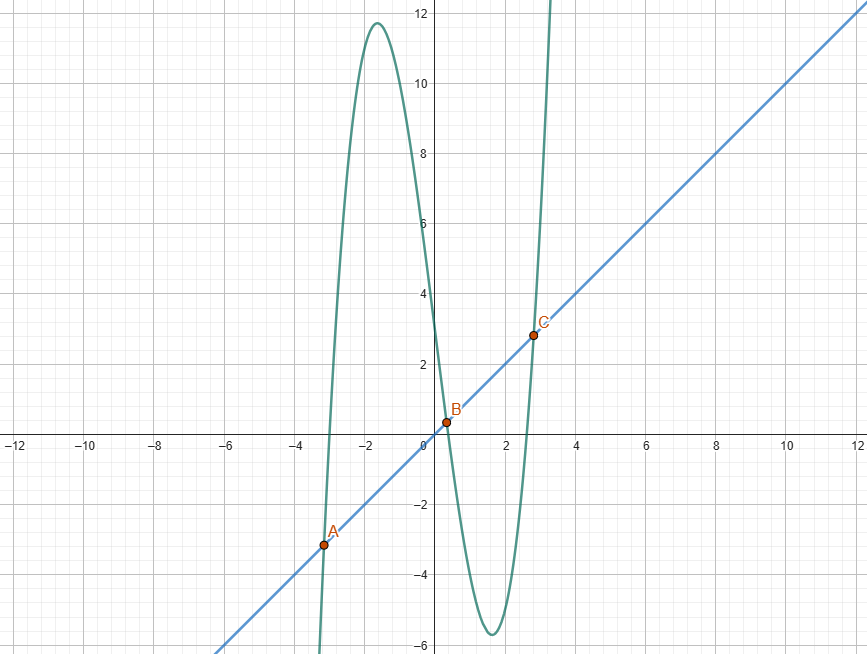
\includegraphics[height = 0.5\textwidth]{Imagens/interseções.png}
    \caption{Interseções entre x e $x^3 - 8x + 3$}
    \label{fig:inters}
\end{figure}

\section{Critério de Parada}
\FIXME{Completar}
\DanielP{gráficos estilo Vera}
O processo é repetido até que a diferença entre duas iterações consecutivas seja inferior a uma tolerância pré-estabelecida %seja vertical (entre o valor da função e o eixo x) ou horizontal (entre o valor da sequência e $\xi$).
ou até que um número máximo de iterações seja atingido.

\begin{itemize} %era pra ficar topificado mesmo?
    \item $|\overline{x} - \xi| < \epsilon$ %x_{k+1} - x_k
    \item $f(\overline{x}) < \epsilon$
\end{itemize}

\LucasM{Definir raiz aproximada}

\section{Método do Ponto Fixo}

O método do ponto fixo \emph{é um método iterativo} que %parte da ideia de que as interseções de duas curvas construídas a partir de uma função f(x) revelam suas raízes para então construir uma função $\varphi(x)$ e buscar suas interseções com a reta identidade, que 
transforma o problema de buscar as raízes de uma função $f(x)$ no problema de encontrar os pontos fixos de uma outra função $\varphi(x)$, denominada de \textbf{função de iteração de ponto fixo}. 
A partir dessa função de iteração, uma sequência é construída recursivamente começando em um valor inicial $x_0$ que convergirá para a raiz $\xi$ de $f(x)$, desde que sejam observadas certas condições sob a função $\varphi(x)$ e o dado inicial $x_0$.

%Após localizar um intervalo que contenha uma raiz pelos métodos expostos,
O primeiro passo é gerar funções de iteração $\varphi$ para $f(x)$, o que pode ser feito isolando $x$ na equação $f(x) = 0$. Por exemplo, manipulando a função $x^3 -9x + 3$  da seguinte forma 
\begin{equation*}
    x^3 - 8x + 3 = x 
\end{equation*} 
obtemos a função de iteração $\varphi(x) = x^3 - 8x + 3$. Com a mesma lógica, outras possíveis funções de iteração para $f$ são

\begin{multicols}{2}
\begin{itemize} %itemize (era enumerate)
    \item[a)] $\varphi_1(x) = \frac{x^3}{9} + \frac{1}{3}$
    \item[b)] $\varphi_2(x) = \sqrt[3]{9x-3}$
    \item[c)] $\varphi_3(x) = \frac{9}{x} - \frac{3}{x^2}$
    \item[d)] $\varphi_4(x) = \sqrt{9 - \frac{3}{x}}$
    \item[e)] $\varphi_5(x) = -\sqrt{9 - \frac{3}{x}}$
    \item[f)] $\varphi_6(x) = x^3 - 8x + 3$
\end{itemize}
\end{multicols}
A forma geral da função de iteração é 
\begin{equation}
    \varphi(x) = x + A(x)f(x) \label{it}
\end{equation}
com $A(\xi) \ne 0$.
%É necessário verificar então se as funções de iteração geradas respeitam essa condição de $A(\xi) \neq 0$. 
Por exemplo, a $\varphi_1(x) = \frac{x^3}{9} + \frac{1}{3}$ na forma geral ficaria 
\begin{equation*}
    \varphi_1(x) = x + \frac{1}{9}f(x)
\end{equation*}
\begin{comment}
    \varphi_1(x) &= x + \frac{1}{9}(x^3 - 9x + 3) \\
    \varphi_1(x) &= x + \frac{x^3}{9} - x + \frac{1}{3} \\
    \varphi_1(x) &= \frac{x^3}{9} + \frac{1}{3}
\end{comment}
em que $A(x) = \frac{1}{9}$. Nesse caso, pode-se observar que A($\xi) \neq 0$.

O resultado a seguir relaciona a raiz de uma função com pontos fixos de uma função de iteração associada a essa função. 

\begin{prop}
Seja $\xi$ uma raiz de uma função $f(x)$ e seja $\varphi(x)$ uma função de iteração associada a $f(x)$. Então, $f(\xi) = 0$ se, e somente se, $\varphi(\xi) = \xi$.
\end{prop}

%Provando primeiramente que a raiz da função é ponto fixo da função de iteração, $f(\xi) = 0 \Rightarrow \varphi(\xi) = \xi$. Começa-se calculando a função de iteração para a raiz $\xi$, isto é, $\varphi(\xi)$, obtendo então, pela forma geral, a raiz somada ao produto da função A pela função original $ \xi + A(\xi)f(\xi)$. Dado que $\xi$ é raiz de f(x), o valor da função calculado em $\xi$ é 0, portanto se tem $\xi + A(\xi) \cdot 0$; o que anula o produto com a função A, $\xi + 0$. Com isso, concluí-se que a função de iteração calculada na raíz é de fato igual a $\xi$.

\begin{proof}
($\Rightarrow$) Pela forma geral da função de iteração temos que $\varphi(\xi) = \xi + A(\xi)f(\xi)$. Uma vez que $f(\xi) = 0$, então $\varphi(\xi) = \xi$.

($\Leftarrow$) Começando novamente pela forma geral da função de iteração, temos que $\varphi(\xi) = \xi + A(\xi)f(\xi)$. Como $\varphi(\xi) = \xi$, concluímos que $A(\xi) f(\xi) = 0$. Tendo como hipótese que $A(\xi) \neq 0$, então $f(\xi) = 0$.
%ou seja, o ponto fixo $\xi$ da função de iteração $\varphi$ é raíz da função original $f(x)$. %q.e.d. (\textit{quod erat demonstrandum}, qual estava-se a demonstrar).
\end{proof}

%\newpage

\LucasM{Aqui, antes de ir para o resultado principal, dar exemplos de funções de iteração que fazem a sequencia convergir e divergir. Inserir gráficos assim como no livro da Vera.} 
\DanielP{ok! uma redemoinho ($\varphi_6$: [$-\sqrt{3}$, $-\sqrt{\frac{7}{3}}$]), uma escadinha($\varphi_1$: [0, $\sqrt{3}$]) e uma divergente($\varphi_4$ e $\varphi_5$; $\varphi_2$ e $\varphi_3$ I)}

Sob condições a respeito da função de iteração, sua derivada e o dado inicial, a convergência da sequência iterativa é garantida, como pode-se observar a seguir.
%Enfim é importante verificar se a função de iteração de ponto fixo respeita as condições para convergência.
\begin{teo} \textbf{Convergência da Sequência Iterativa} \label{teoMPF}\\
    Seja $\xi$ uma raiz de f(x), isolada num intervalo I centrado nessa raiz. Considere uma função de iteração $\varphi(x)$ associada a f(x). Sob as seguintes hipóteses:
    \begin{itemize}
        \item[i)] $\varphi(x)$ e $\varphi'(x)$ são contínuas em I,
        \item [ii)] $|\varphi'(x)| \leq M < 1$ em I,
        \item [iii)] $x_0 \in I$,
    \end{itemize}
    a sequência $x_{k+1} = \varphi(x_k)$ converge para a raiz $\xi$. 
\end{teo}
%Dada uma função $\varphi(x)$ ela é chamada de função de iteração, pois $\varphi(x_k) = x_{k+1}$ e através dessas iterações podemos buscar o ponto fixo dela na qual $x_k = \xi$. Provaremos a seguir que dada uma raíz $\xi$ de f(x) isolada num intervalo I centrado na mesma, a sequência recursiva $\varphi(x_k) = x_{k+1}$ converge para $\xi$ tendo: a função contínua e derivável, e sua derivada também contínua, no intervalo (a,b); o módulo (M) de sua derivada limitado e inferior a unidade no intervalo ($|\varphi'(x)| \leq M < 1$ $\forall x \in (a, b)$); e o primeiro valor da iteração no intervalo ($x_0 \in I$).
\begin{proof}
Como $x_{k+1} = \varphi(x_k)$, subtraindo $\xi$ de ambos os lados da igualdade e usando o fato de que $\varphi(\xi)=\xi$ temos
    \begin{equation}\label{difIt}
        x_{k+1} - \xi = \varphi(x_k) - \varphi(\xi).
    \end{equation}
    Pelo Teorema do Valor Médio (TVM) podemos escrever \\
    \begin{equation}\label{tvm}
        \varphi(x_k) - \varphi(\xi) = \varphi'(c_k) (x_k - \xi)
    \end{equation}
    com $c_k$ entre $x_k$ e $\xi$. Então, substituindo (\ref{tvm}) em (\ref{difIt}), temos
    \begin{align}\label{des}
        %x_{k+1} - \xi &= (x_k - \xi) \ \varphi'(c_k) \\
        |x_{k+1} - \xi| &= |(x_k - \xi) \ \varphi'(c_k)| \nonumber \\
        &= |x_k - \xi| \ |\varphi'(c_k)| \\
        &< |x_k - \xi| \nonumber
    \end{align}
    uma vez que $|\varphi'(x)| < 1$. Como $x_0 \in I$, podemos concluir que $x_k \in I$ para todo $k$ já que, por (\ref{des}), $|x_k - \xi| < |x_0 - \xi|$. 

    Na sequência, provaremos que $x_k$ converge para a raiz $\xi$. Vamos começar mostrando que 
    \begin{equation}\label{lab2}
        |x_1 - \xi| \leq M \ |x_0 - \xi|.
    \end{equation}
    Observe que, como $x_1=\varphi(x_0)$, temos que $x_1 - \xi = \varphi(x_0) - \varphi(\xi)$. Pelo Teorema do Valor Médio temos que $\varphi(x_0) - \varphi(\xi) = (x_0 - \xi) \ \varphi'(c_0)$, para algum $c_0$ entre $x_0$ e $\xi$. Uma vez que $|\varphi'(x)| \leq M$ no intervalo $I$, a seguinte desigualdade é válida
    \begin{align*}
        |x_1 - \xi|&= |x_0 - \xi| \ |\varphi'(c_0)|\\
        &\leq M \ |x_0 - \xi|
    \end{align*}
    e provamos a desigualdade (\ref{lab2}).
    %\begin{align*}
    %    |x_1 - \xi| &= |\varphi(x_0) - \xi| \\
    %    \text{Pelo TVM,} \ \varphi(x_0) - \xi &= (x_0 - \xi) \ \varphi'(c_0) \text{, com $c_0 \in (x_0, \xi)$} \\
    %    |x_1 - \xi| &= |x_0 - \xi| \ |\varphi'(c_0)| \\
    %    \text{Como $|\varphi'(x)| \leq M$,} \ |\varphi'(c_0)| \ |x_0 - \xi| &\leq M \ |x_0 - \xi| \\
    %    |x_1 - \xi| &\leq M \ |x_0 - \xi|
    %\end{align*}
    De modo similar prova-se que $|x_2 - \xi| \leq M \ |x_1 - \xi|$ que, combinado com (\ref{lab2}), implica que $|x_2 - \xi| \leq M^2 \ |x_0 - \xi|$. Repetindo o processo k vezes pode-se concluir que
    \begin{equation}\label{lim0}
        |x_k - \xi| \leq M^k \ |x_0 - \xi|.
    \end{equation}
    Como $0 < M < 1$, se k tende a infinito, $M^k$ tende a 0 e, portanto, $M^k \ |x_0 - \xi|$ também tende a 0. Assim, provamos que
    %\begin{align*}
    %\lim_{k \to \infty} |x_k - \xi| &\leq M^k \ |x_0 - \xi| \\
    %\lim_{k \to \infty} |x_k - \xi| &\leq 0 \ |x_0 - \xi| \\
    %\lim_{k \to \infty} |x_k - \xi| &= 0 \ \text{logo, }
    %\end{align*}
    \begin{equation}
        \lim_{k \to \infty} x_k = \xi, \label{conv.mpf}
    \end{equation}
    ou seja, $x_k$ converge para a raiz.
\end{proof}


% $\varphi'(x) = \frac{x^2}{3}$ \\ $|\varphi'(x)| < 1$ para $x \in (-\sqrt{3}, \sqrt{3})$ 

\subsection{Ordem de convergência}

A ordem de convergência de um método iterativo é uma medida de quão rapidamente a sequência de iterações converge para a solução desejada. Em termos práticos, isso significa que, se um método tem uma ordem de convergência alta, ele será capaz de reduzir mais o erro de aproximação a cada iteração.
\begin{df}
    Seja $\{x_k\}$ uma sequência que converge para $\xi$ e
    \begin{equation} \label{erro}
        e_k = x_k - \xi
    \end{equation}
    o erro na k-ésima iteração.
    %um num. p e uma cte. C
    Se existirem $p > 1$ e $C > 0$ tais que $\lim_{k \to \infty} \frac{|e_{k+1}|}{|e_k|^p} = C$, então $p$ é chamada de \emph{ordem de convergência} da sequência e $C$ é a \emph{constante assintótica de erro}.
\end{df}

\begin{comment} sobre p
A ordem de convergência $p$ de um método iterativo fornece uma informação sobre a rapidez de convergência do processo, pois podemos reescrever (\ref{conv}) como $|e_{k+1}| = C |e_k|^p$ para k tendendo ao infinito. 

Uma vez que a sequência {$x_k$} é convergente, $e_k$ tende a 0 quando $k$ tende ao infinito, portanto, quanto maior for $p$ mais próximo de 0 estará $C|e_k|^p$ (independente de C), implicando numa convergência mais rápida da sequência. Assim, se dois processos iterativos resultam em sequências {$x_k^1$} e {$x_k^2$}, ambas convergindo para $\xi$, com suas respectivas ordens de convergência $p_1$ e $p_2$, se $p_1 > p_2 \geq 1$, o processo que gera a sequência {$x_k^1$} converge mais rapidamente.
\end{comment}
%$|e_{k+1}| \approx C |e_k|^p$
No caso do MPF verificaremos que $p = 1$ portanto a ordem de convergência do método é ao menos linear.
\begin{prop}
    Se 
    \begin{equation}\label{conv}
        \lim_{k \to \infty} \frac{e_{k+1}}{e_k} = C, \ 0 \leq |C| < 1,
    \end{equation}
    então a convergência é pelo menos linear. O MPF tem convergência pelo menos linear.
\end{prop}
\begin{proof}
Partindo de (\ref{difIt}) e (\ref{tvm}), e tomando o  limite com k tendendo a infinito, podemos escrever (\ref{conv}) como
\begin{equation*} %\frac{x_{k+1} - \xi}{x_k - \xi} = \varphi'(c_k)
    \lim_{k \to \infty} \frac{x_{k+1} - \xi}{x_k - \xi} = \lim_{k \to \infty}\varphi'(c_k)
\end{equation*} %se $x_k$ converge para $\xi$ então $c_k$ também converge para $\xi$.
com $c_k$ entre $x_k$ e $\xi$
%, obtendo $C = \varphi'(\xi)$, pois, assim como $x_k$, $c_k$ converge para $\xi$
. %análogo ao uso de (2.4) antes de (2.5), certo?
%é necessário, mostrar que \varphi'(\lim_{k \to \infty} c_k) = \varphi'(\xi)? uma vez que o que importa é que \varphi'(x) < 1 independente do x
Como por hipótese $|\varphi'(x)| < 1$ então $|C| < 1$, portanto, a convergência do MPF é pelo menos linear.
\end{proof}
\newpage
    
%--------------------------------------------------------------------
\section{Método de Newton-Raphson Unidimensional}\label{sec:NR1d}

\TODO{talvez reescrever todas as condições como i) derivada limitada ii) f e g continuas , etc...}

\DanielP{conv quadrática}

\EnzoR{escolhendo a func de iter}

O método de Newton é um caso particular do \textbf{Método do Ponto Fixo} amplamente utilizado para encontrar raízes %\EnzoR{seria raízes complexas, não?} 
reais de funções não lineares, cuja ordem de convergência é pelo menos quadrática. A função de iteração específica para este método produz uma sequência em que cada termo $x_{k+1}$ corresponde, geometricamente, à \textbf{interseção da reta tangente} a $f(x)$ no ponto $(x_k, f(x_k))$ com o eixo x. 

\DanielP{só tem que colocar no lugar certo}
No método do ponto fixo, vimos que se a função satisfaz o Teorema \ref{teoMPF} a sequência $x_{k+1} = \varphi(x_k)$ converge para $\xi$. Além disso, da desigualdade (\ref{lim0}) temos que quanto menor for $|\varphi'(x)|$, mais rápido a sequência $\{x_k\}$ converge.

Aplicando a derivada na forma geral de $\varphi$ pela regra da cadeia obtemos $\varphi'(x) = 1 + A'(x)f(x) + A(x)f'(x)$ e, calculando-a na raiz, obtemos $\varphi'(\xi) = 1 + A(\xi)f'(\xi)$. Usando $\varphi'(\xi) = 0$, concluímos que $A(\xi) = \frac{-1}{f'(\xi)}$. Generalizando, temos $A(x) = \frac{-1}{f'(x)}$. Portanto, desde que $f'(x) \neq 0$, a forma da função de iteração do método de Newton-Raphson é 
\begin{equation} \label{phiNR1d}
    \varphi(x) = x - \frac{f(x)}{f'(x)}.
\end{equation}

Dada uma função \(f(x)\), o processo parte de uma estimativa inicial \(x_0\) e aplica a seguinte fórmula iterativa, a partir da escolha da derivada em (\ref{it})
\begin{equation} \label{nr}
    x_{k+1} = x_k - \frac{f(x_k)}{f'(x_k)},
\end{equation}
onde \(f'(x_k)\) é a derivada da função \(f\) avaliada em \(x_k\).
Para que o método convirja para a raiz correta, é necessário que \(f(x)\) seja continuamente diferenciável em uma vizinhança da raiz e que \(f'(x) \neq 0\) nessa região. Além disso, a escolha adequada do ponto inicial \(x_0\) é crucial para garantir a convergência do método.

\subsection{Interpretação Geométrica}
\DanielP{ficou paia o alinhamento em}
\begin{align*}
    f'(x_0)(x - x_k) &= y - y_k \\
    f'(x_k)(x_{k+1} - x_k) &= -y_k \\
    x_{k+1} - x_k &= \frac{-y_k}{f'(x_k)} \\
    x_{k+1} &= x_k - \frac{y_k}{f'(x_k)}
\end{align*}
\subsection{Convergência}
\begin{teo} \label{teoNR}
    Sejam $f(x)$, $f'(x)$ e $f''(x)$ contínuas num intervalo $I$ que contém a raiz $\xi$ de $f$, supondo $f'(\xi) \neq 0$. Então, existe um intervalo $\overline{I} \subset I$, contendo a raiz $\xi$, tal que $x_0 \in \overline{I}$, a sequência ${x_k}$ gerada pela função de iteração $\varphi(x) = x - \frac{f(x_k)}{f'(x_k)}$ convergirá para a raiz.
\end{teo}
\begin{proof}
    Sendo o método de Newton-Raphson um caso particular do MPF, basta provar que para $\varphi(x) = x - \frac{f(x)}{f'(x)}$ as hipóteses do Teorema \ref{teoMPF} são satisfeitas. 
    
    Primeiramente, observe que 
    \begin{equation} \label{dphiNR}
        \varphi'(x) = \frac{f(x)f''(x)}{[f'(x)]^2}.
    \end{equation}
    Como $f'(\xi) \neq 0$ e $f'(x)$ é contínua em I, é possível obter $I_1 \subset I$ tal que $f'(x) \neq 0$ no intervalo $I_1$. Assim, a função $f$ e suas derivadas primeira e segunda são contínuas em $I_1$ e, consequentemente, a função de iteração e sua derivada também.
    
     Uma vez que a $\varphi'(x)$ é contínua em $I_1$ e $\varphi'(\xi) = 0$, é possível escolher $I_2 \subset I_1$ de modo que $|\varphi'(x)| < 1$ em $I_2$ tendo $\xi$ como centro do novo intervalo.

    Por fim, tomando, $\overline{I} = I_2$, satisfazem-se as hipóteses do Teorema \ref{teoMPF}.
\end{proof}
\subsection{Ordem de Convergência}
No MPF espera-se uma ordem de convergência ao menos linear, entretanto ao escolher uma função de iteração que satisfaça $\varphi'(\xi) = 0$, provaremos que sua ordem de convergência será ao menos quadrática.
\begin{prop}
    A ordem de convergência do método de Newton é pelo menos quadrática.
\end{prop}
\begin{proof}
    Assumiremos todas as hipóteses do Teorema \ref{teoNR}. %(de Convergência do Método de Newton-Raphson), temos
    Partindo de $x_{k+1} = x_k - \frac{f(x_k)}{f'(x_k)}$, subtraindo $\xi$ em ambos os lados da igualdade, obtemos
\begin{equation} \label{eMNR}
    e_{k+1} = e_k - \frac{f(x_k)}{f'(x_k)} 
\end{equation}
O polinômio de Taylor de grau 2 para $f(x)$ centrado em $x_k$ é
\begin{equation*}
    f(x) = f(x_k) + f'(x_k)(x - x_k) + \frac{f''(c_k)}{2}(x-x_k)^2
\end{equation*}
com $c_k$ entre $x$ e $x_k$.
%$-(x-x_k)$
Assim, $f(\xi) = f(x_k) - f'(x_k)(x_k - \xi) + \frac{f''(c_k)}{2}(x_k-\xi)^2$ dado que $f(\xi) = 0$, dividindo a equação pela derivada de $f$ temos, aplicando a fórmula do erro \ref{erro} e a da sequência \ref{nr}
\begin{align*}
    e_k - \frac{f(x_k)}{f'(x_k)} &= \frac{f''(c_k)}{2f'(x_k)}e_k^2 \\
    e_{k+1} &= \frac{f''(c_k)}{2f'(x_k)}e_k^2 \\
    \frac{e_{k+1}}{e_k^2} &= \frac{1}{2} \frac{f''(c_k)}{f'(x_k)}
\end{align*}

Aplicando limite no termo esquerdo da equação acima e, dada a continuidade das funções, nos argumentos à direita, obtemos 
\begin{equation*}
    \lim_{k \to \infty} \frac{e_{k+1}}{e_k^2} = \frac{1}{2} \frac{f''(\xi)}{f'(\xi)}
\end{equation*}
Calculando a $\varphi''$ a partir de $\varphi'$ \ref{dphiNR} %temos $\frac{[f'(x)f''(x)+f(x)f'''(x)][f'(x)]^2 - 2f'(x)f''(x)f(x)f''(x)}{[f'(x)]^4}$, 
em $\xi$ obtemos $\frac{[f'(\xi)]^3f''(\xi)}{[f'(\xi)]^4}$, que é um $C$ concluindo então que a convergência do método de Newton Raphson é ao menos quadrática.
\begin{align*}
    \lim_{k \to \infty} \frac{e_{k+1}}{e_k^2} &= \frac{1}{2} \varphi''(\xi) \\
    &= C
\end{align*}
%\frac{f(x_k)}{f'(x_k)} &= e_k - \frac{f''(c_k)}{2f'(x_k)}e_k^2
\end{proof}
\subsection{Ciladas}
O Método de Newton é amplamente utilizado na prática devido à sua rapidez e precisão em condições ideais. Contudo, em algumas situações ele pode falhar ou convergir para raízes incorretas se essas condições não forem satisfeitas. Estes problemas geralmente estão associados a fatores como: pontos de máximo e mínimo, pontos de inflexão, multiplicidade da raiz e escolha inadequada do chute inicial.

\subsubsection{Alta multiplicidade}
Polinômios de grau elevado tendem a ter alta multiplicidade nas raizes, como no caso do polinômio $x^{10} - 1$.
A convergencia lenta é causada pela multiplicidade da raiz. Quando uma raiz tem multiplicidade $m > 1$ — neste caso $m = 10$ — a derivada próxima a raiz se aproxima de zero, aumentando o número de iterações necessárias para convergir para a raiz.
Isso faz com que a taxa de convergência do metodo de Newton reduza-se para linear em vez da esperada taxa quadrática.
\begin{figure}[H]
    \centering 
    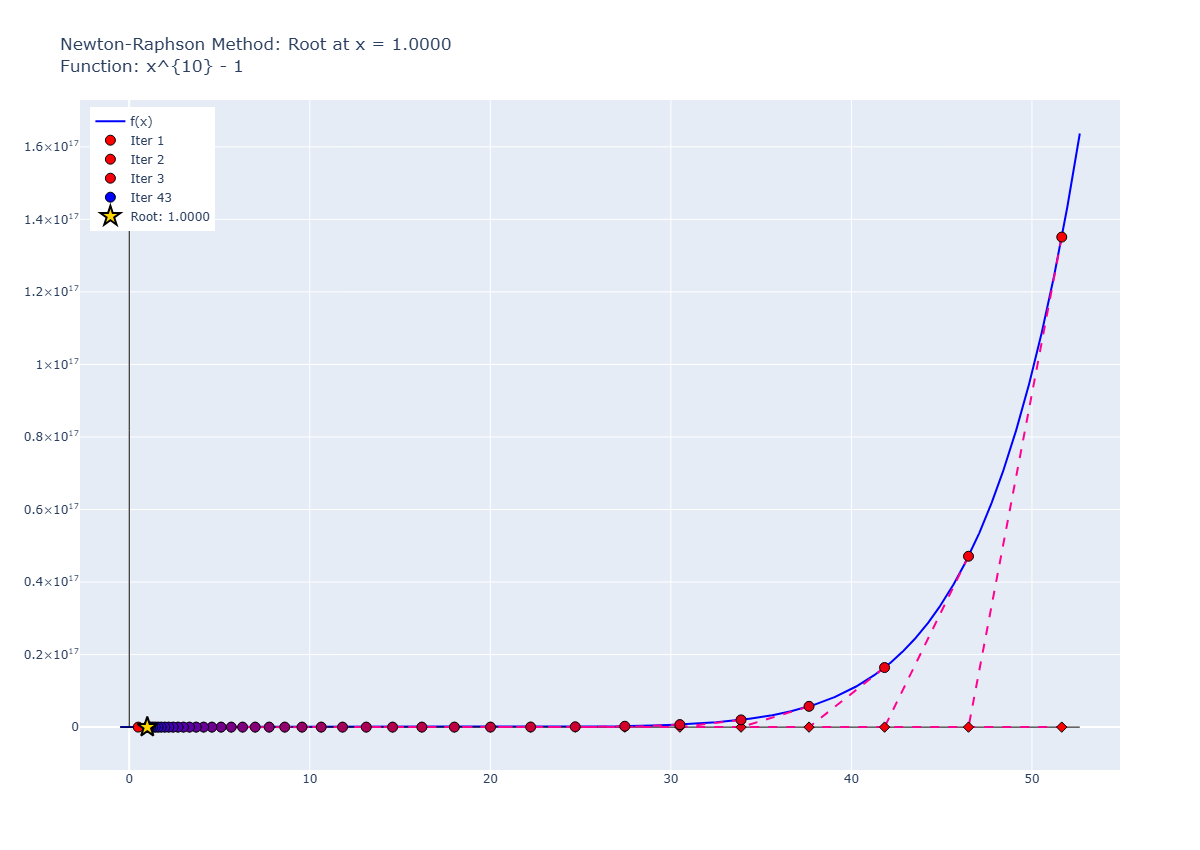
\includegraphics[width=1\textwidth]{Imagens/pitfalls/01/x_10-1.png}
    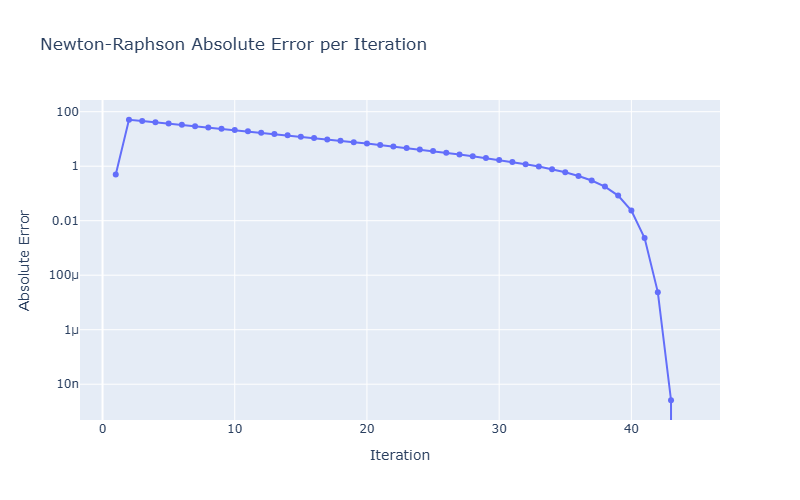
\includegraphics[width=1\textwidth]{Imagens/pitfalls/01/err_x_10-1.png}
    \caption{Gráfico daCilada relacionada a multiplicidade da raiz.}
    \label{fig:ciladaMultRaiz}
\end{figure}

Ao analisar a função geometricamente, é possível observar que a inclinação da tangente à curva em torno da raiz é muito próxima de zero, o que resulta em saltos minúsculos a cada iteração, causando uma convergencia lenta.

\begin{center}
\small
\begin{tabular}{|c|c|c|c|}
\hline
Iteração & Valor de $x_k$ & $f(x)$ & Erro $e_k$ \\
\hline
1 & $x = 0.50000000000000000$ & $f(x) = -0.99902343750000000$ & $0.50000000000000000$ \\
\hline
2 & $x = 51.64999999999999858$ & $f(x) = 135114904483913696$ & $50.64999999999999858$ \\
\hline
3 & $x = 46.48499999999999943$ & $f(x) = 47111654129711536$ & $45.48499999999999943$ \\
\hline
4 & $x = 41.83650000000000091$ & $f(x) = 16426818072478544$ & $40.83650000000000091$ \\
\hline
5 & $x = 37.65285000000000082$ & $f(x) = 5727677301318307$ & $36.65285000000000082$ \\
\hline
$\vdots$ & $\vdots$ & $\vdots$ & $\vdots$ \\
\hline
43 & $x = 1.00000000257760013$ & $f(x) = 0.00000002577600156$ & $0.00000000257760013$ \\
\hline
44 & $x = 1.0$ & $f(x) = 0.0$ & $0.0$ \\
\hline
\end{tabular}
\label{tab:ciladaNR}
\end{center}

\subsubsection{Pontos de extremo}
Outro fator que é um problema quando se trata de taxa de convergência são os pontos de máximo e mínimo da função. Quando uma iteração é iniciada perto de um ponto de máximo ou mínimo um dos problemas que podem ocorrer é a função de iteração convergir para um ponto de máximo ou mínimo ao invés da raiz. Isso pode causar uma diminuição na taxa de convergência.
\begin{figure}[H]
    \centering 
    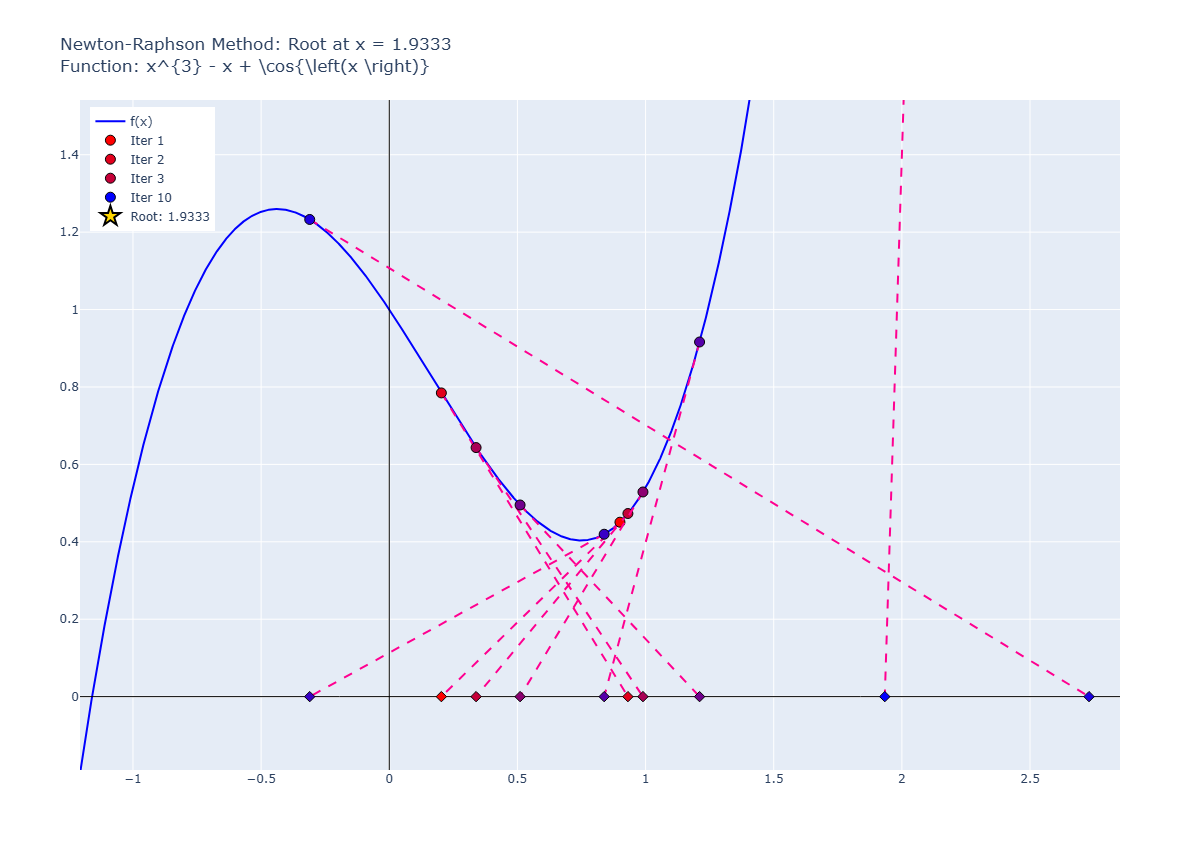
\includegraphics[width=1\textwidth]{Imagens/pitfalls/02/max_min.png}
    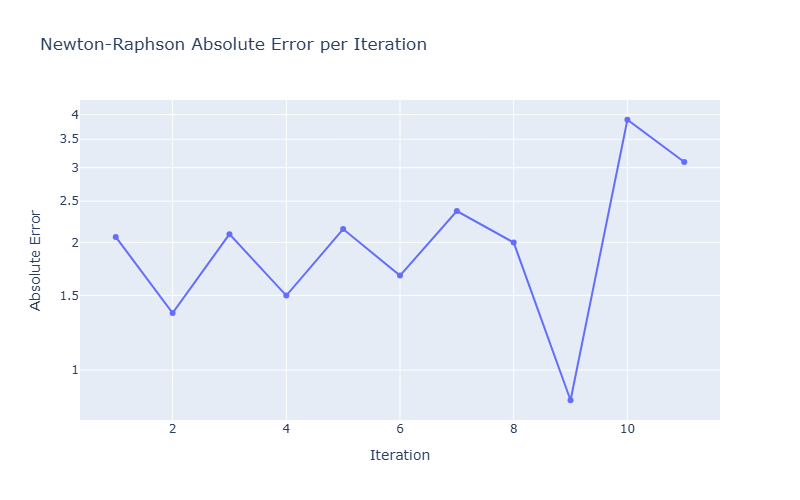
\includegraphics[width=1\textwidth]{Imagens/pitfalls/02/err_max_min.png}
    \caption{Cilada de ponto de Mínimo diminuindo a taxa de convergência.}
    \label{fig:ciladaMinMax_A}
\end{figure}

\begin{center}
\small
\begin{tabular}{|c|c|c|c|}
\hline
Iteração & Valor de $x_k$ & $f(x)$ & Erro $e_k$ \\
\hline
1 & $x = 0.90000000000000002$ & $f(x) = 0.45060996827066446$ & $2.05960580450169983$ \\
\hline
2 & $x = 0.20318738327105890$ & $f(x) = 0.78462959591676906$ & $1.36279318777275882$ \\
\hline
3 & $x = 0.93108680836493152$ & $f(x) = 0.47305585213356149$ & $2.09069261286663144$ \\
\hline
4 & $x = 0.33865524784873213$ & $f(x) = 0.64338650465768399$ & $1.49826105235043205$ \\
\hline
5 & $x = 0.98975277280548202$ & $f(x) = 0.52871601875798535$ & $2.14935857730718194$ \\
\hline
6 & $x = 0.51038365868141022$ & $f(x) = 0.49512408543110442$ & $1.66998946318311026$ \\
\hline
7 & $x = 1.21066335888968579$ & $f(x) = 0.91621158441747408$ & $2.37026916339138571$ \\
\hline
8 & $x = 0.83841140043105933$ & $f(x) = 0.41958113044930967$ & $1.99801720493275914$ \\
\hline
9 & $x = -0.31043606990472872$ & $f(x) = 1.23271962647527022$ & $0.84916973459697120$ \\
\hline
10 & $x = 2.73020451984058488$ & $f(x) = 16.70421900417551697$ & $3.88981032434228480$ \\
\hline
11 & $x = 1.93332993606072678$ & $f(x) = 4.93835804267838796$ & $3.09293574056242671$ \\
\hline
\end{tabular}
\label{tab:ciladaNR}
\end{center}

Em casos extremos, na vizinhança de um ponto de máximo ou mínimo, a intercessão da reta tangente de uma iteração pode coincidir com a coordenada da abscissa da iteração anterior, fazendo com que a sequência não convirja.
\begin{figure}[H]
    \centering 
    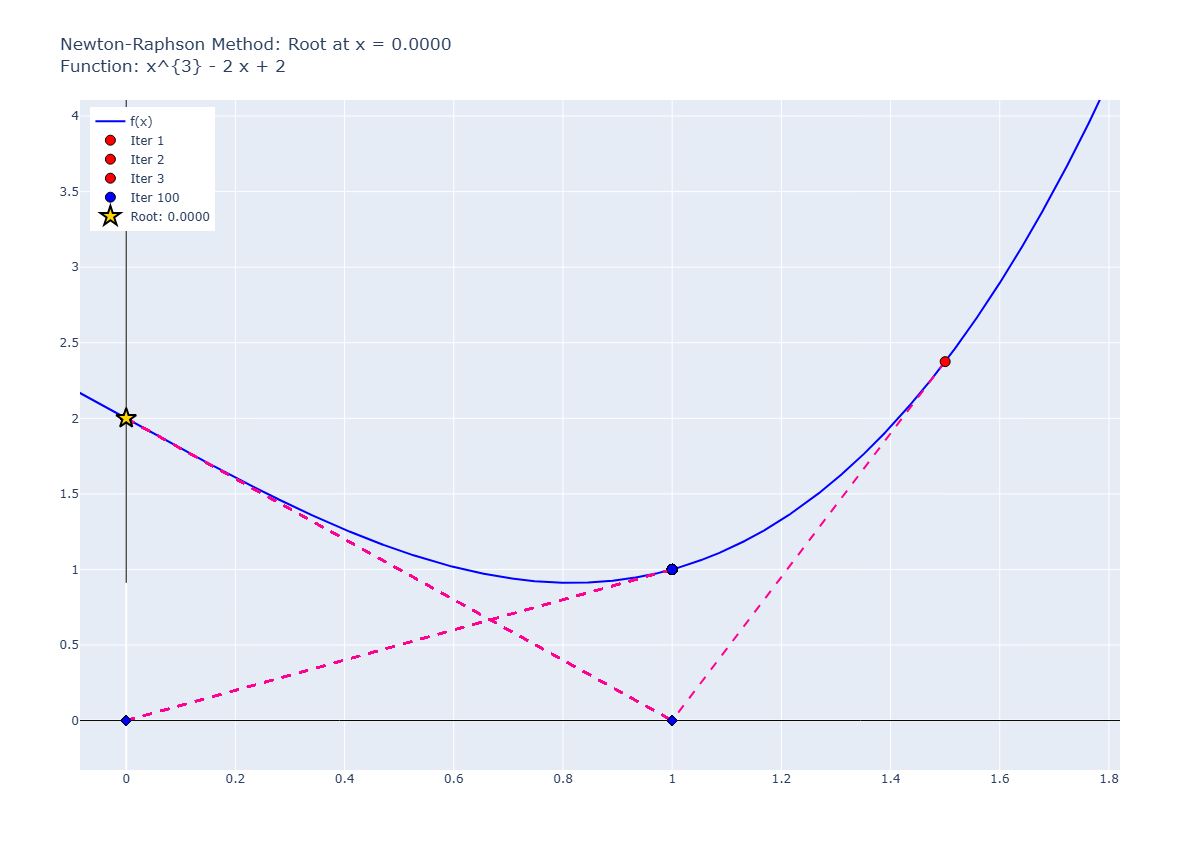
\includegraphics[width=1\textwidth]{Imagens/pitfalls/03/x3_2x_2_10.png}
    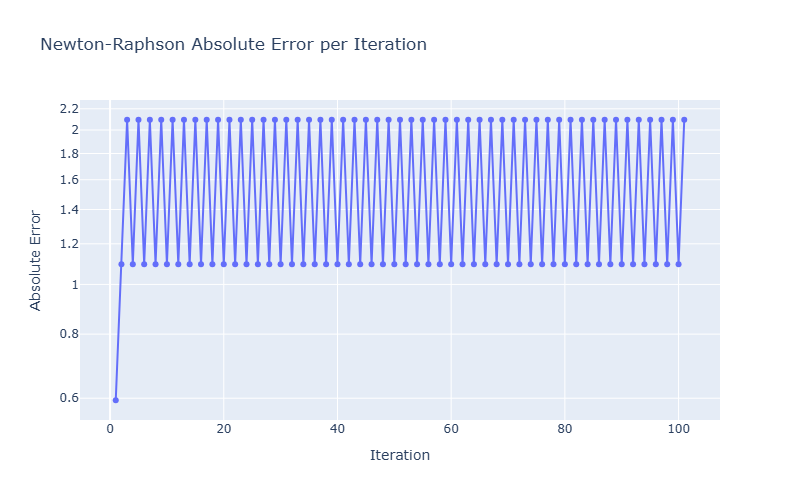
\includegraphics[width=1\textwidth]{Imagens/pitfalls/03/err_x3_2x_2_10.png}
    \caption{Cilada de ponto de Mínimo presa.}
    \label{fig:ciladaMinMax_B}
\end{figure}

\begin{center}
\small
\begin{tabular}{|c|c|c|c|}
\hline
Iteração & Valor de $x_k$ & $f(x)$ & Erro $e_k$ \\
\hline
1 & $x = 1.50000000000000000$ & $f(x) = 2.37500000000000000$ & $0.59455148154232651$ \\
\hline
2 & $x = 1.00000000000000000$ & $f(x) = 1.00000000000000000$ & $1.09455148154232651$ \\
\hline
3 & $x = 0.00000000000000000$ & $f(x) = 2.00000000000000000$ & $2.09455148154232651$ \\
\hline
4 & $x = 1.00000000000000000$ & $f(x) = 1.00000000000000000$ & $1.09455148154232651$ \\
\hline
5 & $x = 0.00000000000000000$ & $f(x) = 2.00000000000000000$ & $2.09455148154232651$ \\
\hline
$\vdots$ & $\vdots$ & $\vdots$ & $\vdots$ \\
\hline
100 & $x = 1.00000000000000000$ & $f(x) = 1.00000000000000000$ & $1.09455148154232651$ \\
\hline
101 & $x = 0.00000000000000000$ & $f(x) = 2.00000000000000000$ & $2.09455148154232651$ \\
\hline
\end{tabular}
\label{tab:ciladaNR}
\end{center}

\subsubsection{Pontos de Inflexão}
Pontos de inflexão também podem causar problemas no método de Newton. Se a raiz estiver próxima de um ponto de inflexão da função \(f(x)\), onde a derivada segunda muda de sinal, o método pode não convergir para a raiz desejada. Isso acontece porque a tangente à curva nesse ponto pode não fornecer uma boa aproximação da raiz, resultando em saltos grandes na iteração e afastando-a da raiz.
\begin{figure}[H]
    \centering 
    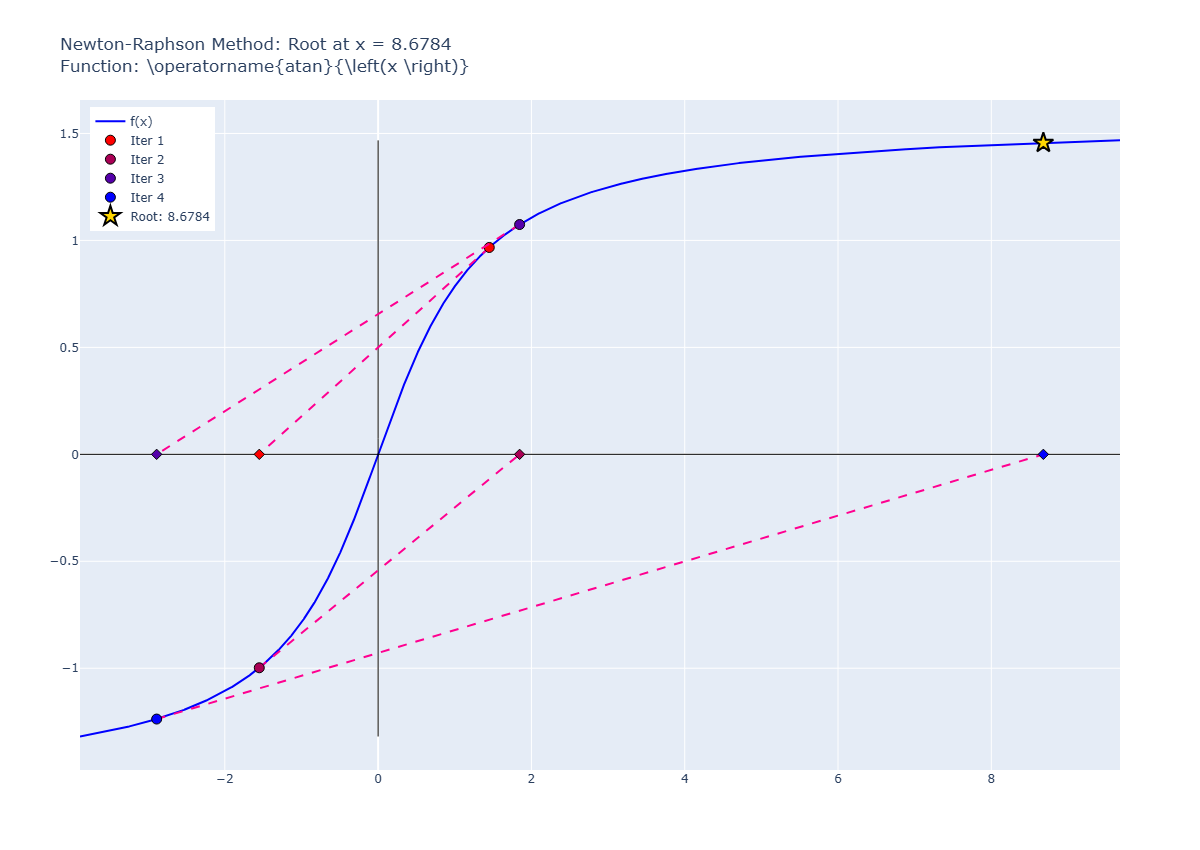
\includegraphics[width=1\textwidth]{Imagens/pitfalls/04/arctg.png}
    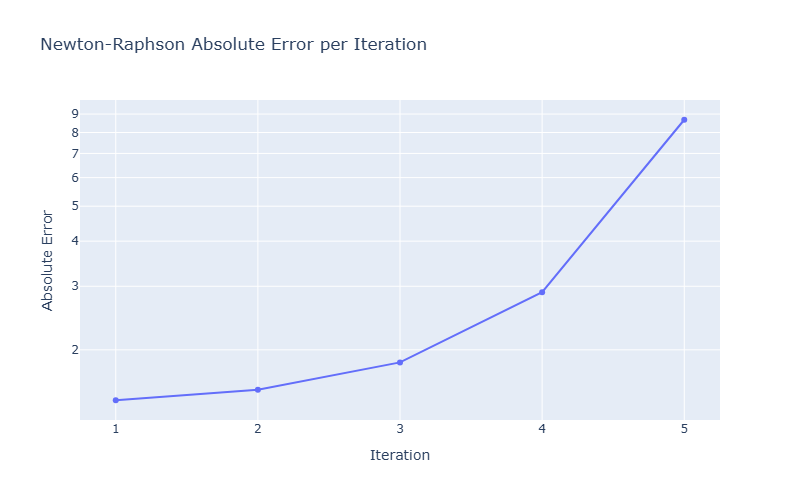
\includegraphics[width=1\textwidth]{Imagens/pitfalls/04/err_arctg.png}
    \caption{Cilada de ponto de Inflexão.}
    \label{fig:ciladaPontoInflexao}
\end{figure}
Ao analisar o gráfico é possivel notar que conforme as iterações avançam, a função se afasta da raiz, resultando em saltos cada vez maiores. Isso ocorre porque a tangente à curva no ponto de inflexão não fornece uma boa aproximação da raiz, levando o método a divergir.

\begin{center}
\small
\begin{tabular}{|c|c|c|c|}
\hline
Iteração & Valor de $x_k$ & $f(x)$ & Erro $e_k$ \\
\hline
1 & $x = 1.44999999999999996$ & $f(x) = 0.96704699339746025$ & $1.44999999999999996$ \\
\hline
2 & $x = -1.55026329701562049$ & $f(x) = -0.99790755802460773$ & $1.55026329701562049$ \\
\hline
3 & $x = 1.84593175119723552$ & $f(x) = 1.07432318743154331$ & $1.84593175119723552$ \\
\hline
4 & $x = -2.88910905408613594$ & $f(x) = -1.23757558204700402$ & $2.88910905408613594$ \\
\hline
5 & $x = 8.67844942653632145$ & $f(x) = 1.45607432393228908$ & $8.67844942653632145$ \\
\hline
\end{tabular}
\label{tab:ciladaNR}
\end{center}

\subsubsection{Derivada próxima de zero}
Além disso, quando a derivada de uma iteração é muito próxima de zero, o metodo vai ter dificuldades em convergir. Isso ocorre porque a divisão por zero ou por um número muito pequeno pode resultar em saltos grandes na iteração, afastando-a da raiz.
\begin{figure}[H]
    \centering 
    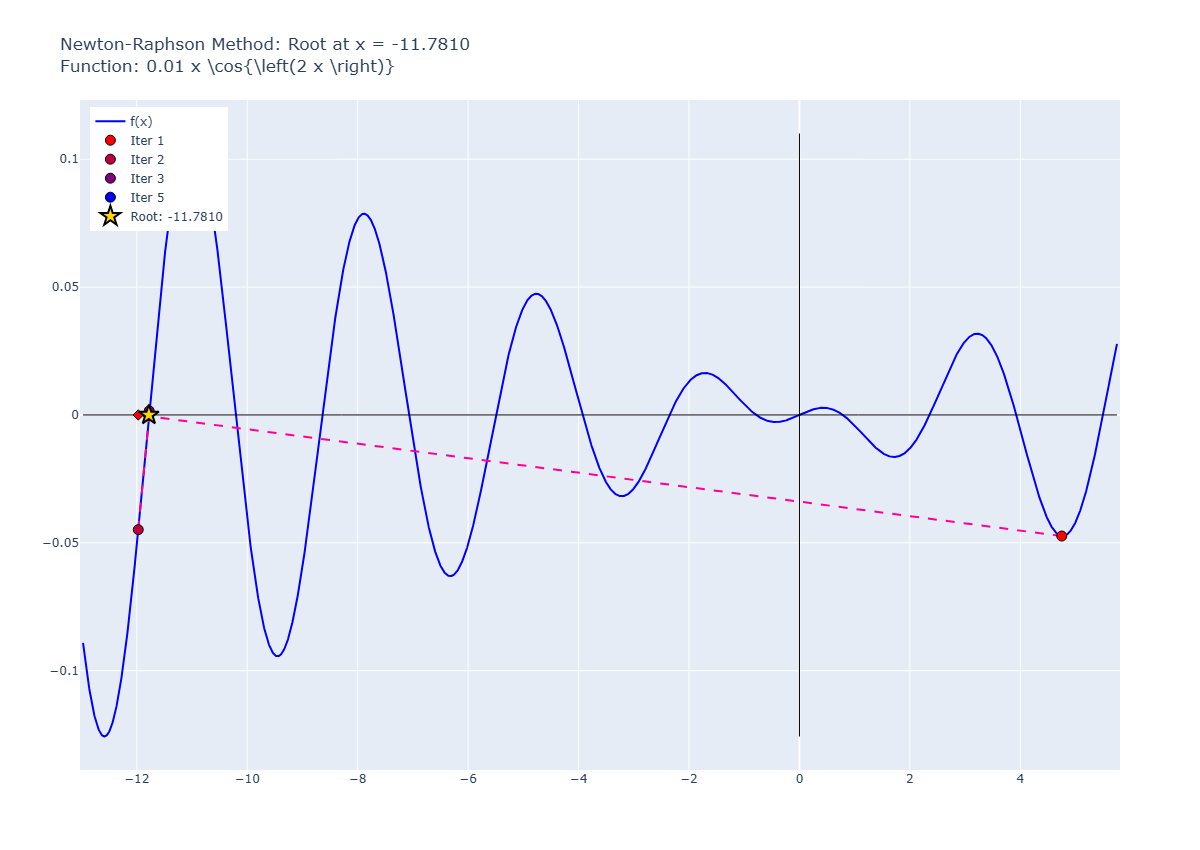
\includegraphics[width=1\textwidth]{Imagens/pitfalls/06/slope_near_zero.png}
    \caption{Cilada de derivada próxima de zero.}
    \label{fig:ciladaDerivadaProximaZero}
\end{figure}
Podemos perceber que a inclinação da tangente à curva em torno da raiz é muito próxima de zero, o que resulta em um salto enorme, levando a iteração para longe da raiz mais próxima.

\begin{center}
\small
\begin{tabular}{|c|c|c|}
\hline
Iteração & Valor de $x_k$ & $f(x)$ \\
\hline
1 & $x = 4.75000000000000000$ & $f(x) = -0.04736567741932798$ \\
\hline
2 & $x = -11.97301255116330410$ & $f(x) = -0.04486365737362013$ \\
\hline
3 & $x = -11.77429070649470333$ & $f(x) = 0.00157340920400228$ \\
\hline
4 & $x = -11.78097664313937010$ & $f(x) = -0.00000098775893849$ \\
\hline
5 & $x = -11.78097245096321544$ & $f(x) = -0.00000000000035126$ \\
\hline
6 & $x = -11.78097245096172507$ & $f(x) = -0.00000000000000010$ \\
\hline
\end{tabular}
\label{tab:ciladaNR}
\end{center}

Em suma, para evitar estes casos, além de analisar o comportamento da função, isto é, analisar pontos de máximo e minimo, derivadas nulas, pontos de inflexão e multiplicidade das raízes, é necessário escolher um bom chute inicial para $x_0$, suficientemente perto da raiz e com uma inclinação da tangente que não seja muito pequena.

\begin{comment}
{Derivada nula:} Se a derivada \(f'(x_k)\) for zero ou muito próxima de zero, a iteração pode divergir ou levar a resultados imprecisos. Isso ocorre porque a divisão por zero ou por um número muito pequeno pode resultar em saltos grandes na iteração, afastando-a da raiz.
{Ponto de inflexão:} Se o ponto inicial \(x_0\) estiver próximo de um ponto de inflexão da função \(f(x)\), onde a derivada muda de sinal, o método pode não convergir para a raiz desejada. Isso acontece porque a tangente à curva nesse ponto pode não fornecer uma boa aproximação da raiz.
{Raízes múltiplas:} Se a função \(f(x)\) tiver uma raiz múltipla, ou seja, uma raiz onde a função toca o eixo x mas não o cruza, o método de Newton pode convergir lentamente ou até mesmo divergir.
{Escolha inadequada de \(x_0\):} Se o ponto inicial \(x_0\) estiver muito longe da raiz ou em uma região onde a função não é bem comportada, o método pode não convergir ou convergir para uma raiz errada. A escolha de um bom ponto inicial é crucial para o sucesso do método
\end{comment}


\section{Método de Newton-Raphson N-dimensional}
O método de Newton-Raphson pode ser estendido para resolver sistemas de equações não lineares em múltiplas variáveis. Um sistema de equações não lineares ser representado da seguinte maneira:
\begin{equation*}
    \begin{cases}
    f_1(x_1, x_2, \ldots, x_n) = 0 \\
    f_2(x_1, x_2, \ldots, x_n) = 0 \\
            \qquad \qquad \vdots \qquad \qquad  \vdots \\
    f_n(x_1, x_2, \ldots, x_n) = 0
    \end{cases}
\end{equation*}
onde  \(f_i \) são as funções não lineares e \(x_i\) são as variáveis desconhecidas.

Podemos escrever esse sistema de \textbf{\(n\)} variáveis como uma função \textbf{\(F : \mathbb{R}^n \rightarrow \mathbb{R}^n\)}' da seguinte forma:
\begin{equation*}
    F((x_1, x_2, \ldots, x_n)) = (f_1(x_1, x_2, \ldots, x_n), f_2(x_1, x_2, \ldots, x_n), \ldots, f_n(x_1, x_2, \ldots, x_n))^{t}
\end{equation*}
Portanto, de forma mais compacta, o sistema pode ser escrito na forma vetorial como \textbf{\(F(X) = 0\)}, onde \textbf{\(F\)} é uma função vetorial e \(X\) é um vetor de variáveis.

\subsection{Definições}

Durante a construção do método de Newton-Raphson unidimensional (\ref{sec:NR1d}), definimos a função de iteração 
\begin{equation*}
\varphi(x) = x - {A(x)}{f(x)}.
\end{equation*}
com isso achamos que a função \(A(x)\) que satisfazia \(\varphi'(\xi) = 0\) é \(A(x) = \frac{-1}{f'(x)}\) desde que \(f'(x) \neq 0\). 
Similarmente, para o caso n-dimensional, generalizamos a função de iteração como
\begin{equation*}
    G(\xb) = x - A(x)^{-1} F(x)
\end{equation*}
em que \(A(x)\) é a matriz não singular que satisfaz \(G'(\xi) = 0\). A matriz \(A(x)\) pode ser representada como
\begin{equation}\label{matA}
    A(x) =  
    \begin{bmatrix}
        a_{11}(x) & a_{12}(x) & \ldots & a_{1n}(x) \\
        a_{21}(x) & a_{22}(x) & \ldots & a_{2n}(x) \\
        \vdots & \vdots & \ddots & \vdots \\
        a_{n1}(x) & a_{n2}(x) & \ldots & a_{nn}(x)
    \end{bmatrix}
\end{equation}
onde cada entrada  \(a_{ij}(x)\) é uma função de   \(\mathbb{R}^n \rightarrow  \mathbb{R}\). Seja \(b_{ij}\) as entradas da matriz inversa \(A^{-1}(x)\). As funções coordenadas  $g_{i}(\xb)$ são da forma

\begin{equation}
    g_{i}(\xb) = x_i - \sum_{j=1}^{n} b_{ij}(x) f_j(x)
\end{equation}
e
\begin{equation}\label{sumInvA}
    \frac{\partial g_i(\xb)}{\partial x_k} = \delta_{ik} - \sum_{j=1}^{n} \left( \frac{\partial b_{ij}(x)}{\partial x_k} f_j(x) + b_{ij}(x) \frac{\partial f_j(x)}{\partial x_k} \right)
\end{equation}
onde \(\delta_{ik}\) é o delta de Kronecker, que é 1 se \(i = k\) e 0 caso contrário.

\subsection{Calculo do Jacobiano}

\newtheorem*{dfNRnd}{Método de Newton-Raphson N-dimensional}
\begin{dfNRnd}
    \begin{prop}
    Seja $\mathbf{p}$ um ponto fixo de \(\mathbb{G}\). Se existe um \(\delta > 0\) tal que

    \begin{itemize} %\label{teoMPF}
        \item[i)] $\frac{\partial g_i}{\partial x_j}$ é contínua em uma vizinhança $N_{\delta} = \{x \in \mathbb{R}^n : ||x - p|| < \delta\}$ para todo $i, j = 1, 2, \ldots, n$
        \item [ii)] $\frac{\partial^2 \mathbb{G}_i}{\partial x_j \partial x_k}$ é contínua e $|\frac{\partial^2g_i(x)}{\partial x_j \partial x_k}| \leq $M$ $
        \item [iii)] $\frac{\partial g_i(p)}{\partial x_k} = 0$, para todo $i = 1,2, \ldots, n$
    \end{itemize}
    Então existe \(\bar{\delta} \leq \delta\) de tal forma que a sequência gerada por $x_{k+1} = \mathbb{G}(x_{k})$ converge para $\mathbf{p}$ de forma quadrática, para qualquer escolha de $x_{0}$ que satisfaz \(|| x_{0} - \mathbf{p} || \leq \bar{\delta}\)
    \end{prop}

\end{dfNRnd}

A demonstração é análoga à do Teorema \ref{teoNR}. E está descrita extensivamente em ref.

A partir de (\ref{sumInvA}) vamos caracterizar a matriz A. Obseve que, de \( \frac{\partial g_i(\mathbf{p})}{\partial x_k} = 0 \) para todo $ i = 1,2, \ldots, n$, temos que
\begin{equation}\label{aInvs1}
    0 = 1 - \sum_{j=1}^{n} \left( b_{ij}(\mathbf{p}) \frac{\partial f_j(\mathbf{p})}{\partial x_i} \right) \ \ \text{para i = j}
\end{equation}
e
\begin{equation}\label{aInvs2}
    0 = - \sum_{j=1}^{n} \left( b_{ij}(\mathbf{p}) \frac{\partial f_j(\mathbf{p})}{\partial x_k} \right)\ \ \text{para i $\neq$ j}.
\end{equation}
A matriz Jacobiana \(J\) de \(F\) é a matriz das derivadas dada a seguir:
\begin{equation}
    J(\mathbf{p}) =
    \begin{bmatrix}
        \frac{\partial f_1(\mathbf{p})}{\partial x_1} & \frac{\partial f_1(\mathbf{p})}{\partial x_2} & \ldots & \frac{\partial f_1(\mathbf{p})}{\partial x_n} \\
        \frac{\partial f_2(\mathbf{p})}{\partial x_1} & \frac{\partial f_2(\mathbf{p})}{\partial x_2} & \ldots & \frac{\partial f_2(\mathbf{p})}{\partial x_n} \\
        \vdots & \vdots & \ddots & \vdots \\
        \frac{\partial f_n(\mathbf{p})}{\partial x_1} & \frac{\partial f_n(\mathbf{p})}{\partial x_2} & \ldots & \frac{\partial f_n(\mathbf{p})}{\partial x_n}
    \end{bmatrix}
\end{equation}
As condições (\ref{aInvs1}) e (\ref{aInvs2}) implicam que
\begin{align*}
    A(\mathbf{p})^{-1} J(\mathbf{p}) &= I \\[6pt]
    A(\mathbf{p}) A(\mathbf{p})^{-1} J(\mathbf{p}) &= A(\mathbf{p}) I \\[6pt]
    I J(\mathbf{p}) &= A(\mathbf{p}) \\[6pt]
    J(\mathbf{p}) &= A(\mathbf{p})
\end{align*}
Portanto, uma escolha natural para \(A(x)\) é a matriz Jacobiana \(J(x)\) de \(F\). Assim, a função de iteração do método de Newton-Raphson n-dimensional é dada por
\begin{equation}
    G(\xb) = x - J(x)^{-1} F(x).
\end{equation}
A sequência iterativa d oMNR n-dimensional é
\begin{equation}\label{seqIterNRndim}
    x_{k+1} = x_k - J(x_k)^{-1} F(x_k)
\end{equation}
onde \(\xb_k\) é a aproximação atual da solução, \(J(x_k)\) é a matriz Jacobiana avaliada em \(x_k\), e \(F(\xb_k)\) é o vetor de funções avaliado em \(x_k\). É esperado que a sequência \(\{x_k\}\) convirja, \textbf{quadraticamente}, para a solução do sistema de equações não lineares, desde que o chute inicial \(x_0\) esteja suficientemente próximo da solução e que a matriz Jacobiana avaliada em \(J(x_k)\) seja invertível nesse ponto.
Vejamos um exemplo para n = 2. Considere o sistema de equações não lineares:
\begin{equation*}
    \begin{cases}
    x^2 + y^2 - 4 = 0 \\
    x^2 - y - 1 = 0
    \end{cases}
\end{equation*}
Podemos definir a função \(F : \mathbb{R}^2 \rightarrow \mathbb{R}^2\) como
\begin{equation*}
    F((x, y)) = \begin{bmatrix}
                    x^2 + y^2 - 4 \\
                    x^2 - y - 1
                \end{bmatrix}
\end{equation*}
A matriz Jacobiana \(J(x, y)\) de \(F\) é dada por
\begin{equation*}
    J((x, y)) = \begin{bmatrix}
        \frac{\partial ( x^2 + y^2 - 4 )}{\partial x} & \frac{\partial ( x^2 + y^2 - 4 )}{\partial y} \\
        \frac{\partial ( x^2 - y - 1 )}{\partial x} & \frac{\partial ( x^2 - y - 1 )}{\partial y}
    \end{bmatrix}
\end{equation*}
\begin{equation*}
    J((x, y)) = \begin{bmatrix}
        2x & 2y \\
        2x & -1
    \end{bmatrix}
\end{equation*}
A iteração do método de Newton-Raphson n-dimensional é então dada por
\begin{align*}
        \begin{bmatrix}
            x_{k+1} \\
            y_{k+1}
        \end{bmatrix} 
        &=
        \begin{bmatrix}
            x_k \\
            y_k
        \end{bmatrix} - J((x_k, y_k))^{-1} F((x_k, y_k)) \\[12pt]
        &=
        \begin{bmatrix}
            x_k \\
            y_k
        \end{bmatrix} - 
        \begin{bmatrix}
            2x_k & 2y_k \\
            2x_k & -1
        \end{bmatrix}^{-1} 
        \begin{bmatrix}
            x_k^2 + y_k^2 - 4 \\
            x_k^2 - y_k - 1
        \end{bmatrix}\\[12pt]
        &=
        \begin{bmatrix}
            x_k \\
            y_k
        \end{bmatrix} - 
        \frac{1}{-2x_k - 4 x_k y_k }
        \begin{bmatrix}
            -1 & -2y_k \\
            -2x_k & 2x_k
        \end{bmatrix} 
        \begin{bmatrix}
            x_k^2 + y_k - 4 \\
            x_k^2 - y_k - 1
        \end{bmatrix}
\end{align*}

Vamos escolher um chute inicial \( (x_0, y_0) = (2, 1) \) e aplicar o método iterativamente:
\begin{center}
\begin{tabular}{|c|c|c|}
\hline
Iteração & $x_k$ & $y_k$ \\
\hline
0 & 2.0000000000000000 & 1.0000000000000000 \\
1 & 1.5000000000000000 & 0.2500000000000000 \\
2 & 1.3095238095238095 & 0.7142857142857143 \\
3 & 1.2727272727272727 & 0.6181818181818182 \\
4 & 1.2679491924311228 & 0.6180339887498950 \\
5 & 1.2679491924311228 & 0.6180339887498950 \\
\hline
\end{tabular}
\end{center}
Após algumas iterações, o método converge para a solução aproximada \( (x, y) \approx (1.2679491924311228, 0.618033988749895) \), que satisfaz o sistema de equações não lineares.

\EnzoR{@LucasM, por favor, verifique se era assim que você desejava.}
Computacionalmente não é interessante fazer o cálculo da inversa da matriz Jacobiana, então podemos reescrever a sequência iterativa (\ref{seqIterNRndim}) criando uma variável auxiliar
\begin{align*}
    \gamma &= - J(x_k)^{-1} F(x_k) \\
    J(x_k) \gamma &= J(x_k) J(x_k)^{-1} F(x_k) \\
    J(x_k) \gamma &= - F(x_k) \label{auxNRndim}
\end{align*}
Subistituindo $\gamma$ em ( \ref{seqIterNRndim} ) temos
\begin{equation*}
    x_{k+1} = x_k + \gamma
\end{equation*}

\newpage

\subsection{Fractais de Newton}
A aplicação do método de Newton para os pontos do \textit{\textbf{Plano Complexo}} gera os \textbf{Fractais de Newton}.
\begin{figure}[H]
    \centering
    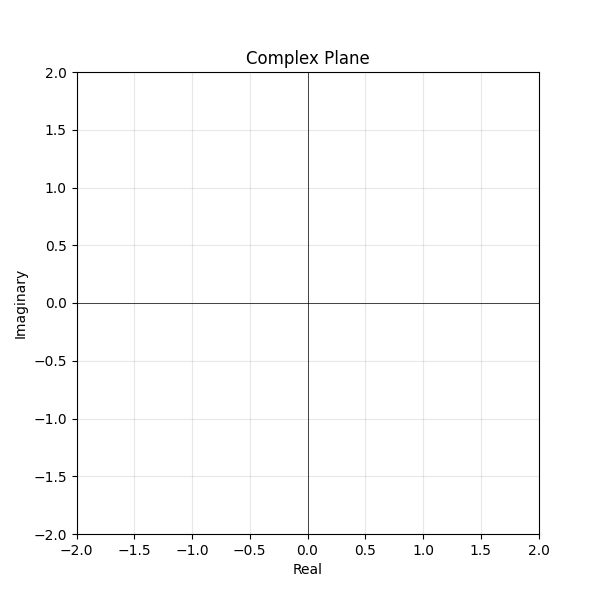
\includegraphics[width=1\textwidth]{Imagens/complexPlane/complex_plane_axes.png}
    \caption{Plano Complexo}
    \label{fig:complexPlane}
\end{figure}
\begin{figure}[H]
    \centering
    \begin{minipage}{0.48\textwidth}
        \centering
        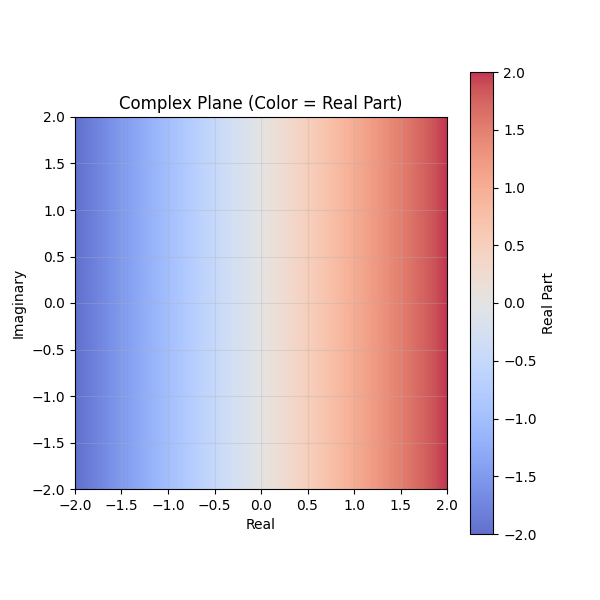
\includegraphics[width=\textwidth]{Imagens//complexPlane/complex_plane_real_part.png}
        \caption*{Parte Real}
    \end{minipage}\hfill
    \begin{minipage}{0.48\textwidth}
        \centering
        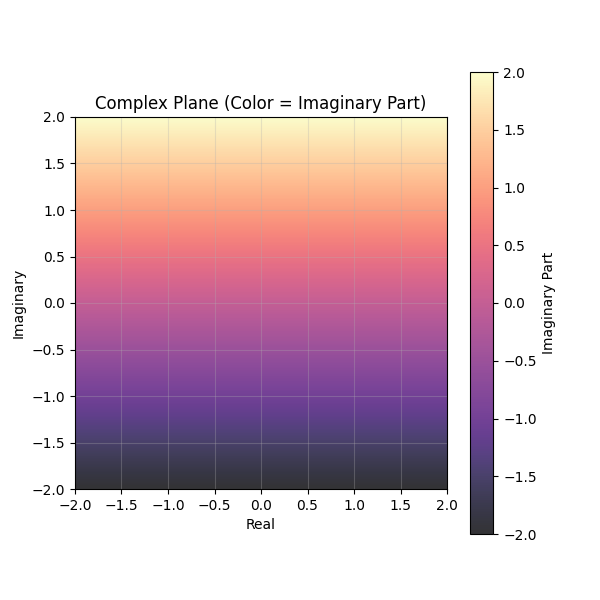
\includegraphics[width=\textwidth]{Imagens//complexPlane/complex_plane_imaginary_part.png}
        \caption*{Parte Imaginária}
    \end{minipage}\\[1em]
    \begin{minipage}{0.48\textwidth}
        \centering
        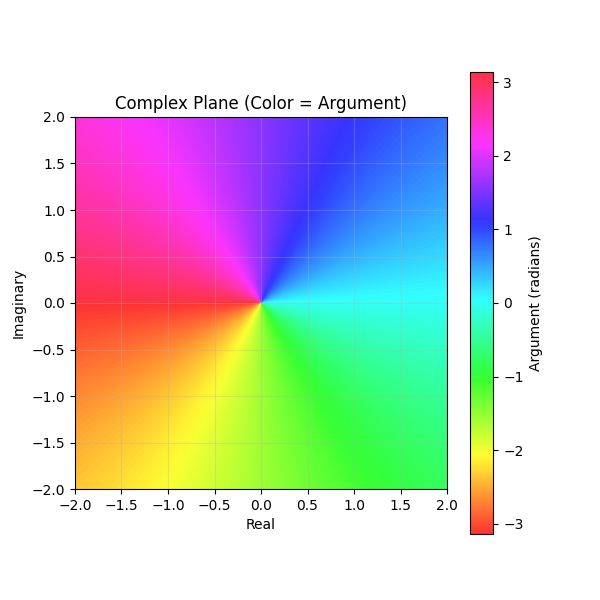
\includegraphics[width=\textwidth]{Imagens//complexPlane/complex_plane_argument.png}
        \caption*{Parte Angular}
    \end{minipage}\hfill
    \begin{minipage}{0.48\textwidth}
        \centering
        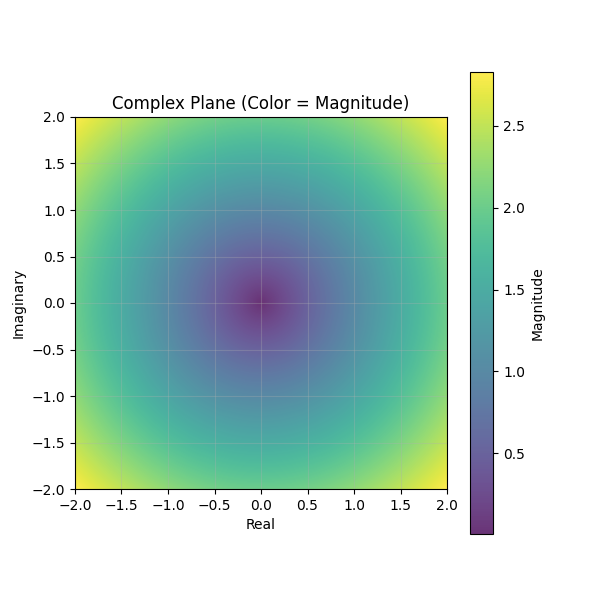
\includegraphics[width=\textwidth]{Imagens//complexPlane/complex_plane_magnitude.png}
        \caption*{Parte Magnitude}
    \end{minipage}
    \caption{Propriedades dos Números Complexos}
    \label{fig:complexPlaneProps}
\end{figure}
O método de Newton-Raphson no plano complexo é aplicado a funções complexas \(f: \mathbb{C} \rightarrow \mathbb{C}\). A fórmula de iteração é semelhante à do caso real, mas agora \(z\) é um número complexo:
\begin{equation*}
    z_{n+1} = z_n - \frac{f(z_n)}{f'(z_n)}
\end{equation*}
onde \(z_n\) é a aproximação atual, \(f(z_n)\) é o valor da função no ponto \(z_n\), e \(f'(z_n)\) é a derivada da função no ponto \(z_n\).

asdklsahdoisahop
A ideia básica para gerar um fractal de Newton é aplicar o método de Newton-Raphson a cada ponto em uma região do plano complexo e colorir o ponto com base na raiz para a qual ele converge e o número de iterações que levou para convergir. Se um ponto não convergir para nenhuma raiz dentro da tolerância estabelecida, ele é colorido de uma forma diferente. Nos gráficos utilizados nessa seção, quanto mais escura uma cor, mais tempo levou para convergir, e preto indica que não convergiu.

\begin{figure}[H]
    \centering 
    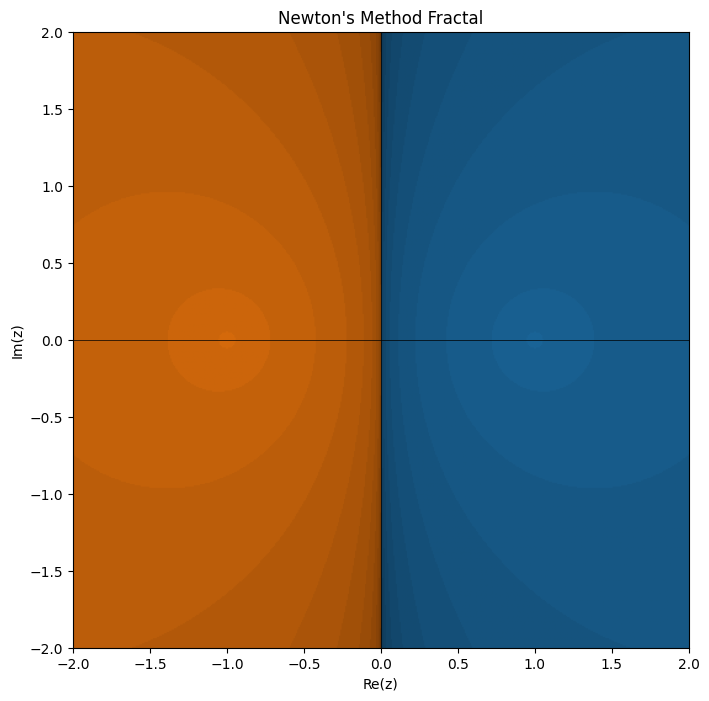
\includegraphics[width=1\textwidth]{Imagens/nr2d_fractals/unit_roots/unitroot2.png}
    \caption{Fractais de Newton -- 2 Unidades da raiz.}
    \label{fig:fractaisnr_unitroots2}
\end{figure}


\begin{figure}[H]
    \centering 
    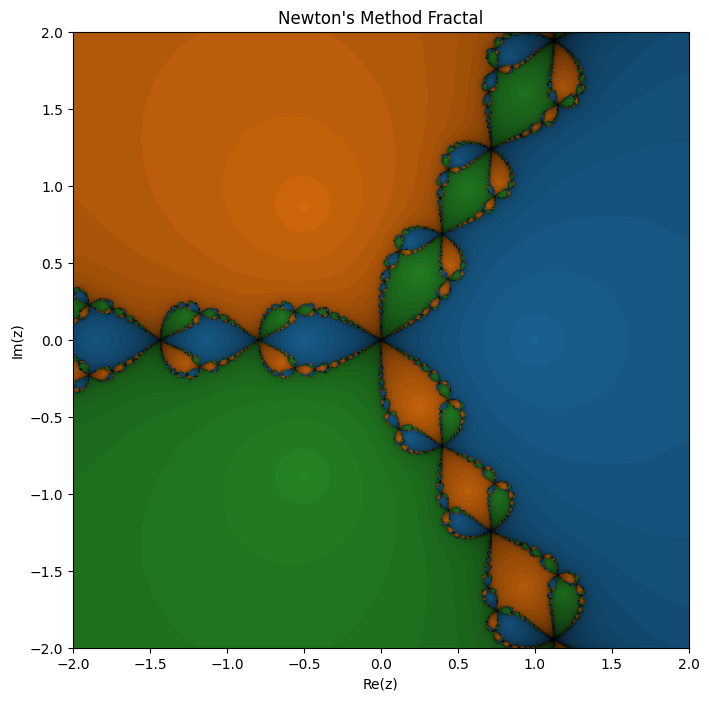
\includegraphics[width=1\textwidth]{Imagens/nr2d_fractals/unit_roots/unitroot3.png}
    \caption{Fractais de Newton - 3 Unidades da raiz.}
    \label{fig:fractaisnr_unitroots3}
\end{figure}


\begin{figure}[H]
    \centering 
    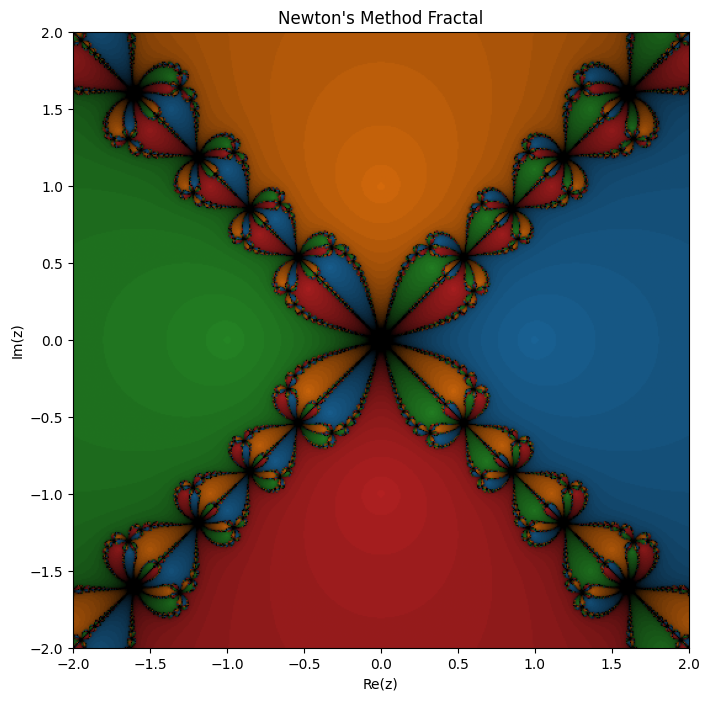
\includegraphics[width=1\textwidth]{Imagens/nr2d_fractals/unit_roots/unitroot4.png}
    \caption{Fractais de Newton - 4 Unidades da raiz.}
    \label{fig:fractaisnr_unitroots4}
\end{figure}


\begin{figure}[H]
    \centering 
    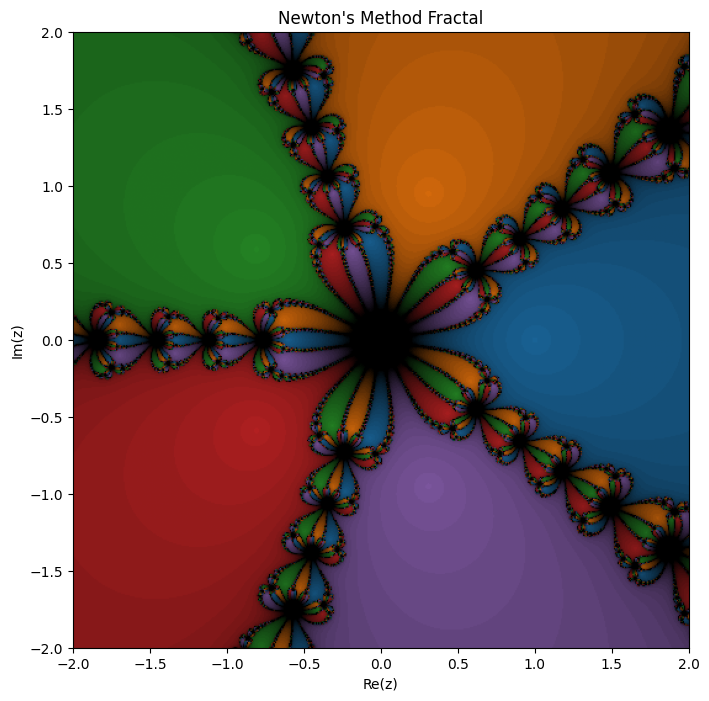
\includegraphics[width=1\textwidth]{Imagens/nr2d_fractals/unit_roots/unitroot5.png}
    \caption{Fractais de Newton - 5 Unidades da raiz.}
    \label{fig:fractaisnr_unitroots5}
\end{figure}


\begin{figure}[H]
    \centering
    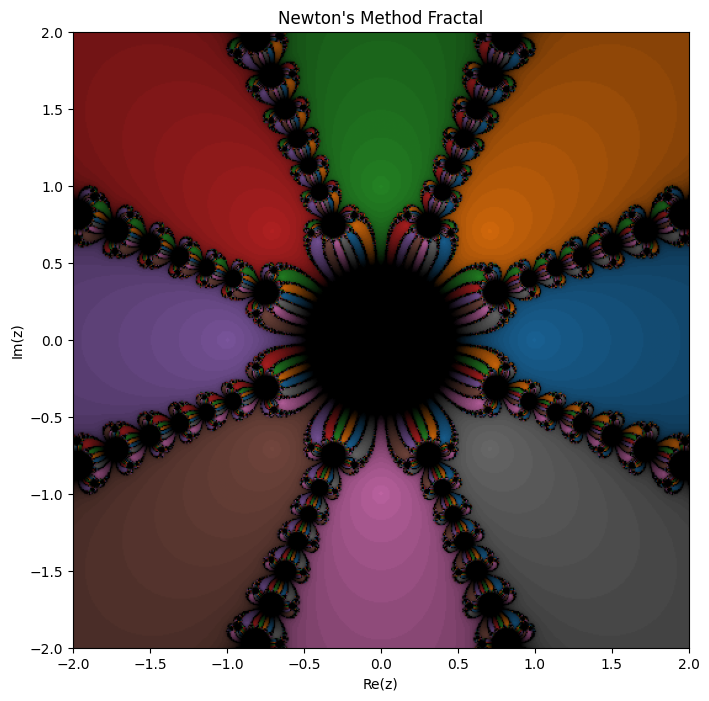
\includegraphics[width=1\textwidth]{Imagens/nr2d_fractals/unit_roots/unitroot8.png}
    \caption{Fractais de Newton - 8 Unidades da raiz.}
    \label{fig:fractaisnr_unitroots8}
\end{figure}


\begin{figure}[H]
    \centering
    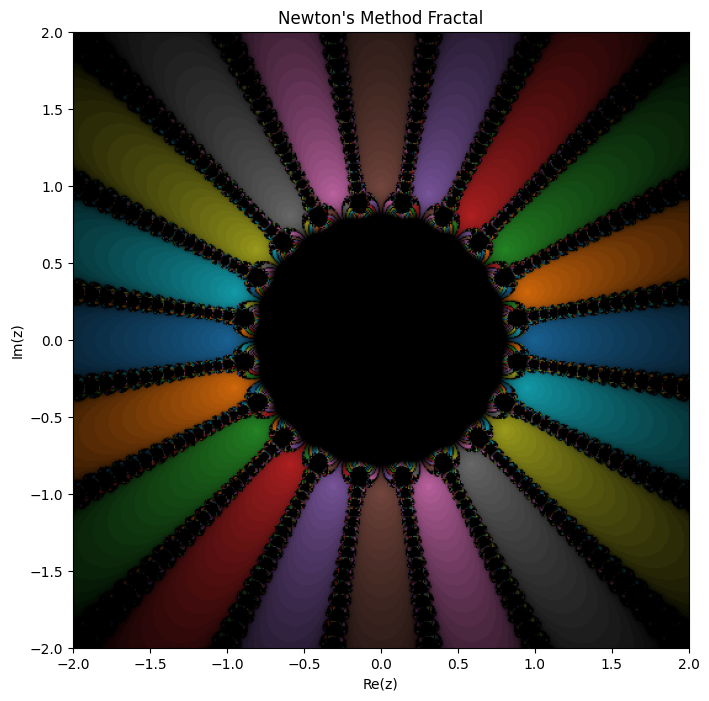
\includegraphics[width=1\textwidth]{Imagens/nr2d_fractals/unit_roots/unitroot20.png}
    \caption{Fractais de Newton - 20 Unidades da raiz.}
    \label{fig:fractaisnr_unitroots20}
\end{figure}

\begin{figure}[H]
    \centering
    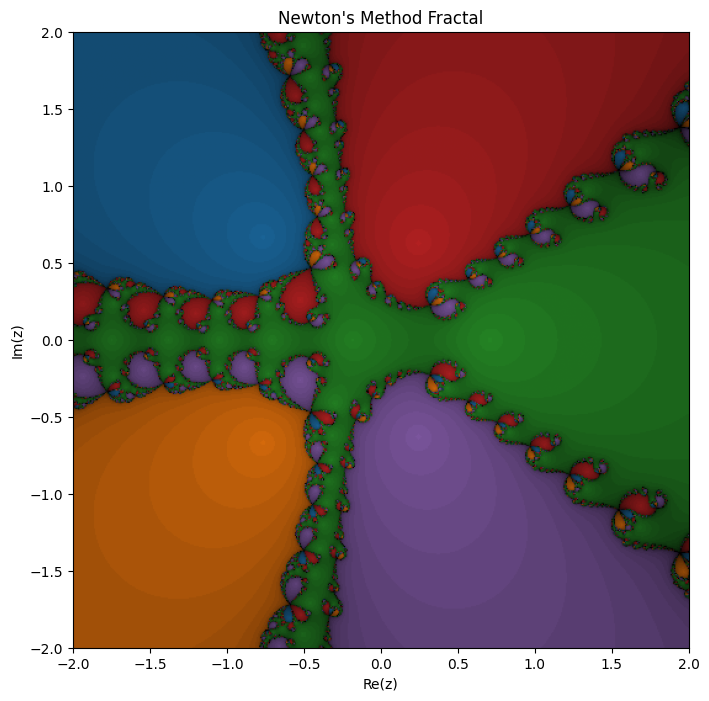
\includegraphics[width=1\textwidth]{Imagens/nr2d_fractals/polinomials/nrfractal_polinomio.png}
    \caption{Fractais de Newton - Polinomio ABCD.}
    \label{fig:fractaisnr_polinomials1}
\end{figure}

\begin{figure}[H]
    \centering
    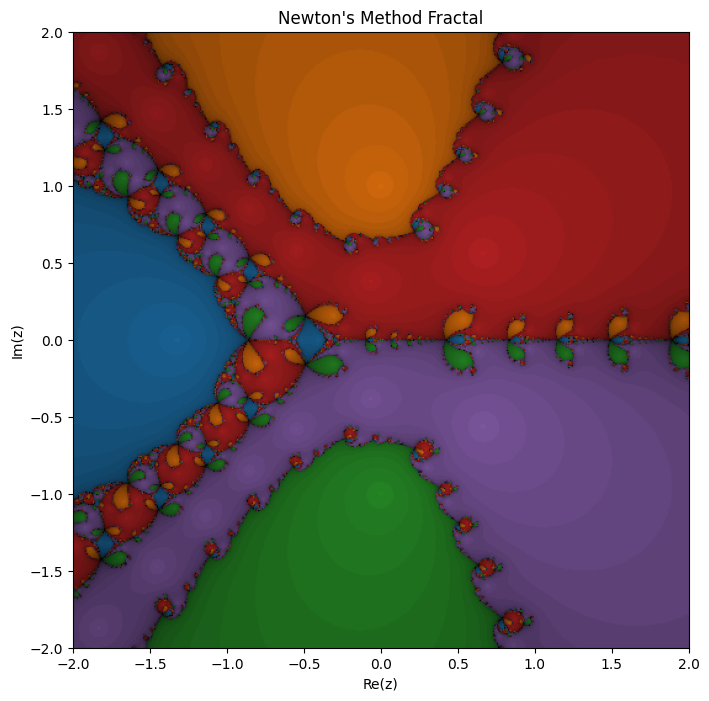
\includegraphics[width=1\textwidth]{Imagens/nr2d_fractals/polinomials/nrfractal_polinomio2.png}
    \caption{Fractais de Newton - Polinomio ABCD.}
    \label{fig:fractaisnr_polinomials1}
\end{figure}

\begin{figure}[H]
    \centering
    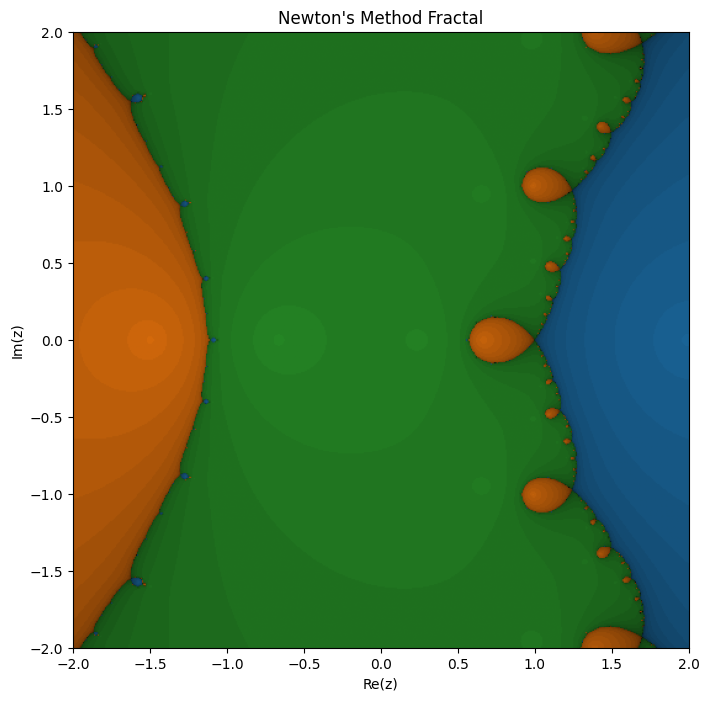
\includegraphics[width=1\textwidth]{Imagens/nr2d_fractals/polinomials/nrfractal_polinomio3.png}
    \caption{Fractais de Newton - Polinomio ABCD.}
    \label{fig:fractaisnr_polinomials1}
\end{figure}

\begin{figure}[H]
    \centering
    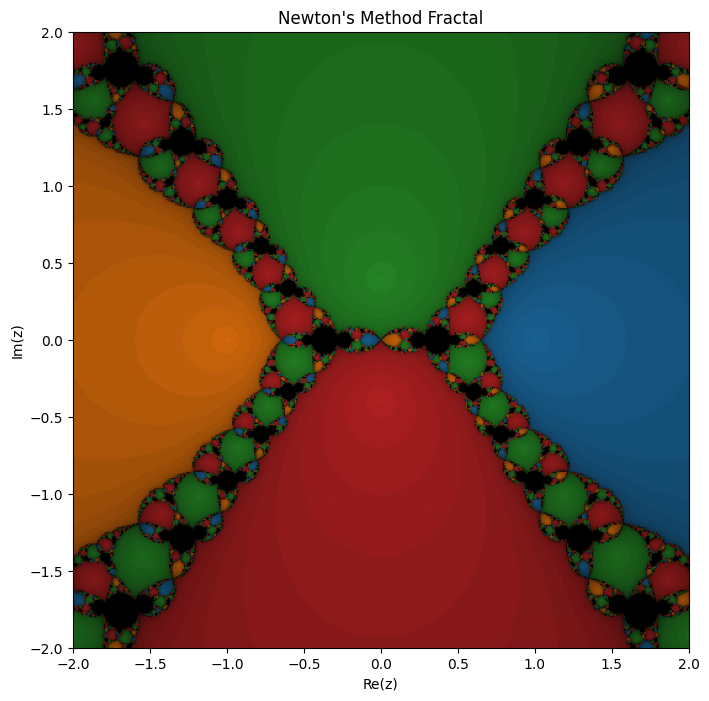
\includegraphics[width=1\textwidth]{Imagens/nr2d_fractals/polinomials/nrfractal_polinomio4.png}
    \caption{Fractais de Newton - Polinomio ABCD.}
    \label{fig:fractaisnr_polinomials1}
\end{figure}



\section{Aplicações}
O método de Newton-Raphson é amplamente utilizado em diversas áreas da ciência e engenharia devido à sua eficiência e rapidez na convergência para soluções de equações não lineares. Algumas das principais aplicações incluem:    
\begin{itemize}
    \item \textbf{Engenharia Elétrica:} Utilizado para análise de fluxo de carga em sistemas de energia elétrica, ajudando a determinar as tensões e correntes em diferentes pontos da rede.
    \item \textbf{Mecânica Estrutural:} Empregado na análise de estruturas não lineares, como pontes e edifícios, para calcular deformações e tensões sob cargas variadas.
    \item \textbf{Economia:} Aplicado na resolução de modelos econômicos complexos que envolvem múltiplas variáveis interdependentes, como equilíbrio geral e otimização de recursos.
    \item \textbf{Ciência da Computação:} Usado em algoritmos de aprendizado de máquina e otimização, especialmente em redes neurais para ajustar pesos e minimizar funções de custo.
    \item \textbf{Física:} Utilizado na simulação de sistemas físicos não lineares, como dinâmica de fluidos e mecânica quântica, para resolver equações diferenciais complexas.
    \item \textbf{Química:} Empregado na modelagem de reações químicas e equilíbrio químico, ajudando a prever concentrações de reagentes e produtos.
\end{itemize}
